% ============================================================
% Grockers Online Shopping Store - ICT Website Project Report
% Deliverable 1: Planning and Analysis  (CSC-114, Bahria University Islamabad)
% Compile with: pdflatex report.tex  (run twice for the table of contents)
% Overleaf: upload this single file, set compiler to pdfLaTeX.
% ============================================================
\documentclass[10pt,a4paper]{article}

\usepackage[a4paper,top=2.3cm,bottom=2.0cm,left=2cm,right=2cm,headheight=14pt]{geometry}
\usepackage[T1]{fontenc}
\usepackage[utf8]{inputenc}
\usepackage[scaled=0.95]{helvet}
\renewcommand{\familydefault}{\sfdefault}
\usepackage[table]{xcolor}
\usepackage{tikz}
\usepackage{array,tabularx,booktabs,float}
\usepackage{enumitem}
\usepackage{caption}
\usepackage{fancyhdr}
\usepackage{titlesec}
\usepackage[hidelinks]{hyperref}

% ---------- colours ----------
\definecolor{gkgreen}{HTML}{2E7D32}
\definecolor{gkdark}{HTML}{1B5E20}
\definecolor{gkaccent}{HTML}{F9A825}
\definecolor{gkbg}{HTML}{F5F5F5}
\definecolor{gktext}{HTML}{212121}
\color{gktext}

% ---------- headings ----------
\titleformat{\section}{\Large\bfseries\color{gkgreen}}{\thesection}{0.6em}{}[\vspace{-0.5ex}\color{gkgreen}\titlerule]
\titleformat{\subsection}{\normalsize\bfseries\color{gkdark}}{\thesubsection}{0.6em}{}
\titlespacing*{\section}{0pt}{1.4ex plus 0.5ex}{1.2ex}
\titlespacing*{\subsection}{0pt}{1.6ex plus 0.5ex}{0.8ex}

% ---------- header / footer ----------
\pagestyle{fancy}
\fancyhf{}
\lhead{\small Grockers Website Project}
\rhead{\small CSC-114 $|$ Deliverable 1}
\lfoot{\small Group Code Miners $|$ Bahria University, Islamabad}
\rfoot{\small Page \thepage}
\renewcommand{\headrulewidth}{0.4pt}
\renewcommand{\footrulewidth}{0.4pt}
\setlength{\parindent}{0pt}
\setlength{\parskip}{0.5ex}

% ---------- tables ----------
\newcolumntype{Y}{>{\raggedright\arraybackslash}X}
\newcommand{\hc}[1]{\textcolor{white}{\bfseries #1}}
\newcommand{\tbl}{\rowcolors{2}{white}{gkbg}\renewcommand{\arraystretch}{1.2}\footnotesize}
\captionsetup{font=small,labelfont={bf,color=gkdark},skip=3pt}
\captionsetup[table]{position=top,skip=3pt}
\setlist{itemsep=0.2ex,topsep=0.3ex,leftmargin=1.3em}

% ---------- wireframe drawing helpers ----------
\tikzset{
  wfbox/.style={draw=black!70,fill=white,line width=0.3pt,align=center},
  wffill/.style={draw=black!60,fill=gray!25,line width=0.3pt,align=center},
  wfbtn/.style={draw=gkdark,fill=gkgreen,text=white,line width=0.3pt,align=center},
  wftext/.style={align=center},
  wfbold/.style={align=center,font=\bfseries},
  wflbl/.style={align=left},
  wfinput/.style={draw=black!45,fill=white,text=black!60,line width=0.3pt,align=left},
}
\newcommand{\wb}[9]{\node[#5,anchor=south west,inner sep=0.4pt,minimum width=#3cm,minimum height=#4cm,text width=#8cm,font=\fontsize{#6}{#7}\selectfont] at (#1cm,#2cm) {#9};}

\begin{document}

% ====================== TITLE PAGE ======================
\begin{titlepage}
\thispagestyle{empty}
\begin{tikzpicture}[remember picture,overlay]
  \fill[gkgreen] (current page.north west) rectangle ([yshift=-3.6cm]current page.north east);
  \fill[gkaccent] ([yshift=-3.6cm]current page.north west) rectangle ([yshift=-3.85cm]current page.north east);
\end{tikzpicture}
\vspace*{-1.2cm}
\begin{center}
{\color{white}\Large\bfseries BAHRIA UNIVERSITY, ISLAMABAD CAMPUS\\[3pt]
\normalsize DEPARTMENT OF COMPUTER SCIENCE}

\vspace{3.6cm}
{\fontsize{30}{36}\selectfont\bfseries\color{gkgreen} Grockers Online\\Shopping Store}

\vspace{0.6cm}
{\Large ICT Website Project Report}

\vspace{0.3cm}
{\Large\bfseries\color{gkdark} Deliverable 1: Planning and Analysis}

\vspace{1.4cm}
\renewcommand{\arraystretch}{1.5}
\begin{tabular}{r@{\hspace{1.2em}}l}
\textbf{Course} & Introduction to Information and Communication Technology (CSC-114)\\
\textbf{Semester} & Fall 2026, BS (CS) Semester 1\\
\textbf{Project phase} & 1 (Planning and Analysis)\\
\textbf{Group name} & Code Miners\\
\textbf{Instructor} & Ms.\ Nadia Kalsoom\\
\end{tabular}

\vspace{1cm}
{\large\bfseries\color{gkgreen} Group Members}\\[4pt]
\renewcommand{\arraystretch}{1.35}
\begin{tabular}{lc}
\toprule
\textbf{Name} & \textbf{Enrollment ID}\\
\midrule
Ghulam Qadir & 01-134262-147\\
Asaam Abdullah & 01-134262-106\\
Armish Malik & 01-134262-020\\
\bottomrule
\end{tabular}

\vspace{1.2cm}
\textbf{GitHub repository:}\\
\href{https://github.com/Armishmalik/CodeMiners.git}{\textcolor{gkgreen}{\texttt{https://github.com/Armishmalik/CodeMiners.git}}}

\vspace{0.8cm}
\textbf{Submission date:} 19 November 2026
\end{center}
\end{titlepage}

% ====================== FRONT MATTER ======================
\begin{table}[H]
\centering
\caption{Version history of this report}
\tbl
\begin{tabularx}{\textwidth}{@{}llYl@{}}
\rowcolor{gkgreen}\hc{Version} & \hc{Date} & \hc{Changes} & \hc{Author(s)}\\
1.0 & 19/11/2026 & Chapters 1--3: introduction, requirements, planning and design & All members\\
\end{tabularx}
\end{table}

\begingroup
\renewcommand{\contentsname}{Contents}
\small
\tableofcontents
\endgroup

% ====================== CHAPTER 1 ======================
\section{Introduction}

\subsection{Organisation Background and Problem Statement}
Grockers is an emerging local online grocery and household-essentials marketplace that serves urban communities. Our group, \textbf{Code Miners}, acts as a small web-development company that plans and builds the Grockers website. At present Grockers sells mainly through physical storefronts and scattered social-media pages. Customers cannot easily see what is in stock or what it costs, and staff answer the same questions again and again. This costs the business sales and wastes the time of both customers and staff. Table~\ref{tab:problems} lists the main problems, their impact and the website feature that addresses each one.

\textbf{Problem statement:} Grockers needs one mobile-friendly website where customers can find products and prices, contact the store and prepare an order.

\begin{table}[H]
\centering
\caption{Problems of the current situation, their impact and the proposed solution}\label{tab:problems}
\tbl
\begin{tabularx}{\textwidth}{@{}cY Y Y@{}}
\rowcolor{gkgreen}\hc{No.} & \hc{Problem} & \hc{Impact} & \hc{Proposed website solution}\\
1 & No central product catalogue. Stock, prices and categories can only be checked in the store or by scrolling social-media posts. & Customers cannot compare items quickly and may shop elsewhere, so sales are lost. & Products page with categories and price tables (FR4).\\
2 & No inquiry or feedback channel. There is no digital way to ask questions, give feedback or request bulk orders. & Communication is delayed and staff repeat the same answers. & Contact page with a validated inquiry form (FR7) and a Services page (FR5).\\
3 & Not usable on mobile devices. There is no responsive platform, although most customers use smartphones for quick local lookups. & Customer reach is limited; reading or ordering on a phone is slow. & Responsive layout using Flexbox/Grid and media queries (NFR3).\\
4 & No online ordering or customer accounts. Orders are placed by phone or in person. & Repeat customers re-enter details every time; phone orders are error-prone. & Cart page, Login and Sign-Up pages, simulated in the browser (FR8, FR9).\\
\end{tabularx}
\end{table}

\subsection{Project Objectives}
The primary, measurable objectives of the project are listed in Table~\ref{tab:objectives}.

\begin{table}[H]
\centering
\caption{Project objectives and measures of success}\label{tab:objectives}
\tbl
\begin{tabularx}{\textwidth}{@{}cY Y@{}}
\rowcolor{gkgreen}\hc{ID} & \hc{Objective} & \hc{Measure of success}\\
O1 & Build a user-friendly, responsive website of 9 pages using HTML5, CSS3 and JavaScript, with the same navigation bar and footer on every page. & All 9 pages complete and linked by the final deliverable on 10 December 2026.\\
O2 & Provide a catalogue of grocery products with structured details and a pricing table. & Products page reachable from Home in at most 3 clicks (Home $\rightarrow$ Products is 1 click).\\
O3 & Make the layout work from phone to desktop screens and keep pages fast. & No sideways scrolling at 360, 768, 1280 and 1920 px; every page loads in under 2 seconds on standard broadband.\\
O4 & Apply good web-development practice: semantic markup, alt text for every image, a label for every form field, consistent styling. & No errors in the W3C HTML and CSS validators.\\
O5 & Demonstrate core ICT concepts: client--server architecture, internet protocols and data security. & Each concept explained in the final report and shown in the demo (see Section~\ref{sec:ict}).\\
O6 & Work as a team using Git and GitHub. & Every member makes at least 10 commits to the repository.\\
\end{tabularx}
\end{table}

\subsection{Target Users}
\begin{table}[H]
\centering
\caption{Target user groups}\label{tab:users}
\tbl
\begin{tabularx}{\textwidth}{@{}lYl@{}}
\rowcolor{gkgreen}\hc{User group} & \hc{Needs} & \hc{Main pages}\\
Customers: students, hostel residents, working adults and families & Browse grocery products and prices; place orders from a phone or computer. & Home, Products, Cart, Login\\
Store owner and staff & Show correct products, prices and contact information; receive customer inquiries. & Products, Services, Contact\\
First-time visitors & Learn about Grockers, its services and how to contact it. & Home, About, Services, Gallery, Contact\\
\end{tabularx}
\end{table}

\subsection{Scope}
The project covers the planning, design and front-end simulation of a responsive website for Grockers with \textbf{exactly 9 pages}: Home, About, Products, Services, Gallery, Contact, Cart, Login and Sign-Up.

\begin{table}[H]
\centering
\caption{Project scope}\label{tab:scope}
\tbl
\begin{tabularx}{\textwidth}{@{}YY@{}}
\rowcolor{gkgreen}\hc{In scope} & \hc{Out of scope in this phase}\\
Planning, design and front-end build of the 9 pages & Back-end server and real database\\
Responsive layout (360--1920 px) with Flexbox/Grid and media queries & Real user accounts and password storage\\
JavaScript form validation, cart and simulated Login/Sign-Up & Stock control, order fulfilment and delivery tracking\\
Hosting on GitHub Pages and version control on GitHub & \\
\end{tabularx}
\end{table}
\textbf{Assumptions:} product data is written directly in the HTML/JavaScript files, and images are sample photographs prepared by the team.

% ====================== CHAPTER 2 ======================
\section{Requirements Analysis}

\subsection{Functional Requirements}
\begin{table}[H]
\centering
\caption{Functional requirements (FR)}\label{tab:fr}
\tbl
\begin{tabularx}{\textwidth}{@{}clYl@{}}
\rowcolor{gkgreen}\hc{ID} & \hc{Page} & \hc{Requirement} & \hc{Priority}\\
FR1 & All pages & A navigation bar and footer must appear on all 9 pages for seamless switching. & Must\\
FR2 & Home & Promotional banners and quick links to the top categories. & Must\\
FR3 & About & The Grockers story, mission and vision, with a store image. & Should\\
FR4 & Products & Items grouped by category, with descriptions and a pricing table. & Must\\
FR5 & Services & Delivery options and packaging standards. & Must\\
FR6 & Gallery & Optimised store-setup and product photographs. & Should\\
FR7 & Contact & Interactive inquiry form with validation, plus store location, phone and hours. & Must\\
FR8 & Cart & Add and remove items, change quantities and view the order total. & Must\\
FR9 & Login, Sign-Up & Simulated authentication and registration in the browser (JavaScript only). & Should\\
FR10 & Forms & JavaScript checks for empty fields, e-mail format and matching passwords. & Must\\
\end{tabularx}
\end{table}

\subsection{Non-Functional Requirements}
\begin{table}[H]
\centering
\caption{Non-functional requirements (NFR)}\label{tab:nfr}
\tbl
\begin{tabularx}{\textwidth}{@{}cl Y Y@{}}
\rowcolor{gkgreen}\hc{ID} & \hc{Category} & \hc{Requirement} & \hc{How it will be checked}\\
NFR1 & Performance & Pages load within 2 seconds on standard broadband; images are compressed. & Network tab of browser developer tools.\\
NFR2 & Readability & High-contrast colours and clear typography (16 px base text). & Contrast checker and peer review.\\
NFR3 & Responsiveness & Layout adjusts to mobile, tablet and desktop widths using Flexbox/Grid and media queries. & Device mode at 360, 768, 1280 and 1920 px.\\
NFR4 & Accessibility & Alt text on every image, a label on every form field, text contrast of at least 4.5:1. & W3C validators and contrast checker.\\
NFR5 & Privacy & Form data is handled without exposing sensitive credentials; passwords are never shown in plain text or committed to the repository. & Code review.\\
NFR6 & Compatibility & Works in the latest Chrome, Firefox and Edge. & Manual test in each browser.\\
NFR7 & Maintainability & One shared CSS file and shared JavaScript files, with comments and consistent file names. & Code review.\\
\end{tabularx}
\end{table}

\subsection{User Stories}
\begin{table}[H]
\centering
\caption{User stories with acceptance criteria}\label{tab:us}
\tbl
\begin{tabularx}{\textwidth}{@{}cYYl@{}}
\rowcolor{gkgreen}\hc{ID} & \hc{User story} & \hc{Acceptance criterion} & \hc{Links to}\\
US1 & As a customer, I want to see products with their prices in a table, so that I can compare items before ordering. & Each category lists item, weight, unit price and an Add to Cart button. & FR4\\
US2 & As a hostel student, I want to ask about bulk supply through the contact form, so that I get a clear reply from the store. & Form with name, e-mail and message; error shown if a field is empty or the e-mail is invalid. & FR7, FR10\\
US3 & As a customer using a phone, I want pages that fit my small screen, so that I can shop quickly while travelling. & Every page is readable at 360 px with no sideways scrolling. & NFR3\\
US4 & As a customer, I want to see my cart total before confirming, so that I know how much I must pay. & Cart shows subtotal, delivery and total estimate, updated when a quantity changes or an item is removed. & FR8\\
US5 & As a returning customer, I want to log in to my account, so that I do not have to enter my details again for every order. & Registered e-mail and password give a logged-in state; wrong details give an error message. & FR9, FR10\\
\end{tabularx}
\end{table}

\subsection{ICT Requirements}\label{sec:ict}
\begin{table}[H]
\centering
\caption{ICT requirements of the user}
\tbl
\begin{tabularx}{\textwidth}{@{}lY@{}}
\rowcolor{gkgreen}\hc{Item} & \hc{Requirement}\\
Hardware & Smartphone, tablet, laptop or desktop computer with a screen at least 360 px wide.\\
Operating system & Android, iOS, Windows, macOS or Linux (any recent version).\\
Browser & Latest Chrome, Firefox, Edge or Safari with JavaScript turned on.\\
Internet connection & Stable mobile data or Wi-Fi connection of at least 1 Mbps.\\
\end{tabularx}
\end{table}

\begin{table}[H]
\centering
\caption{ICT requirements of the organisation (computer setup to maintain the site)}
\tbl
\begin{tabularx}{\textwidth}{@{}lY@{}}
\rowcolor{gkgreen}\hc{Item} & \hc{Requirement}\\
Hardware & One laptop or desktop (at least 8 GB RAM) for updating the site, and a phone for testing.\\
Software & Visual Studio Code, a browser with developer tools, Git and the W3C validators.\\
Operating system & Windows 10/11 or Linux on the maintenance computer.\\
Internet connection & Reliable broadband connection to upload changes to GitHub.\\
Hosting and domain & Free hosting on GitHub Pages for this project; a paid domain name may be added later.\\
Security and backup & Strong GitHub passwords, HTTPS provided by the host, and regular backups of the website files.\\
\end{tabularx}
\end{table}

\textbf{ICT concepts the project demonstrates:}
\begin{itemize}
\item \textbf{Client--server architecture and HTTP/HTTPS:} the visitor's browser (client) requests pages from the GitHub Pages server, which sends back HTML, CSS and JavaScript files over HTTPS.
\item \textbf{URLs and DNS:} the site address is resolved by the Domain Name System to the hosting server.
\item \textbf{Data security:} HTTPS encryption, strong passwords, input validation, and no passwords or secrets stored in the repository.
\item \textbf{Version control:} Git commits and GitHub keep a history of every change and allow safe teamwork.
\end{itemize}

% ====================== CHAPTER 3 ======================
\section{Planning and Design}

\subsection{Site Map Architecture}
The website has nine interconnected pages (Figure~\ref{fig:sitemap}). Every page shares one navigation bar and footer (FR1), so any page can be reached from any other in one click. Products are added to the cart from the Products page, and Login and Sign-Up link to each other.

\begin{center}
\resizebox{\textwidth}{!}{%
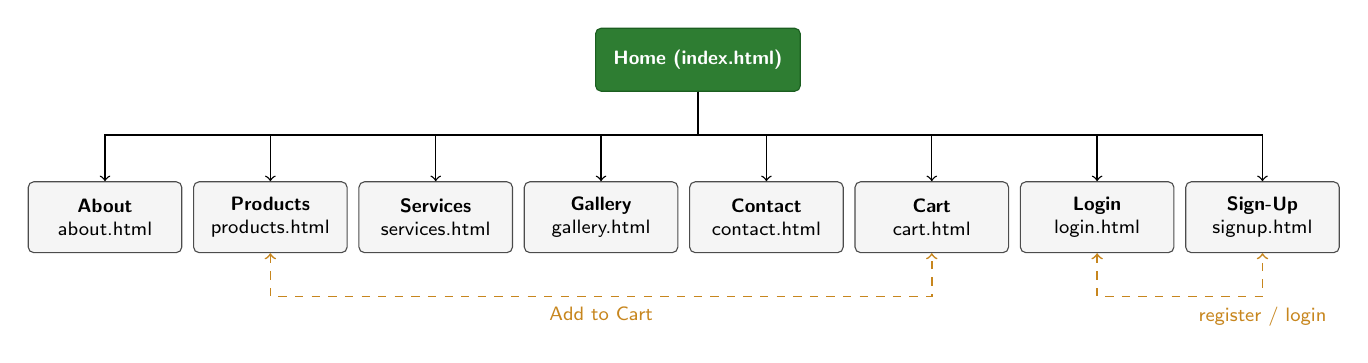
\begin{tikzpicture}[node distance=0,every node/.style={font=\scriptsize\sffamily}]
\node[draw=gkdark,fill=gkgreen,text=white,minimum width=2.6cm,minimum height=0.8cm,rounded corners=2pt] (home) at (8.5,0) {\bfseries Home (index.html)};
\node[draw=black!70,fill=gkbg,minimum width=1.95cm,minimum height=0.9cm,rounded corners=2pt,align=center] (n0) at (0.97,-2) {\bfseries About\\about.html};
\draw[->,line width=0.5pt] (home.south) -- ++(0,-0.55) -| (n0.north);
\node[draw=black!70,fill=gkbg,minimum width=1.95cm,minimum height=0.9cm,rounded corners=2pt,align=center] (n1) at (3.07,-2) {\bfseries Products\\products.html};
\draw[->,line width=0.5pt] (home.south) -- ++(0,-0.55) -| (n1.north);
\node[draw=black!70,fill=gkbg,minimum width=1.95cm,minimum height=0.9cm,rounded corners=2pt,align=center] (n2) at (5.17,-2) {\bfseries Services\\services.html};
\draw[->,line width=0.5pt] (home.south) -- ++(0,-0.55) -| (n2.north);
\node[draw=black!70,fill=gkbg,minimum width=1.95cm,minimum height=0.9cm,rounded corners=2pt,align=center] (n3) at (7.27,-2) {\bfseries Gallery\\gallery.html};
\draw[->,line width=0.5pt] (home.south) -- ++(0,-0.55) -| (n3.north);
\node[draw=black!70,fill=gkbg,minimum width=1.95cm,minimum height=0.9cm,rounded corners=2pt,align=center] (n4) at (9.37,-2) {\bfseries Contact\\contact.html};
\draw[->,line width=0.5pt] (home.south) -- ++(0,-0.55) -| (n4.north);
\node[draw=black!70,fill=gkbg,minimum width=1.95cm,minimum height=0.9cm,rounded corners=2pt,align=center] (n5) at (11.47,-2) {\bfseries Cart\\cart.html};
\draw[->,line width=0.5pt] (home.south) -- ++(0,-0.55) -| (n5.north);
\node[draw=black!70,fill=gkbg,minimum width=1.95cm,minimum height=0.9cm,rounded corners=2pt,align=center] (n6) at (13.57,-2) {\bfseries Login\\login.html};
\draw[->,line width=0.5pt] (home.south) -- ++(0,-0.55) -| (n6.north);
\node[draw=black!70,fill=gkbg,minimum width=1.95cm,minimum height=0.9cm,rounded corners=2pt,align=center] (n7) at (15.67,-2) {\bfseries Sign-Up\\signup.html};
\draw[->,line width=0.5pt] (home.south) -- ++(0,-0.55) -| (n7.north);
\draw[<->,dashed,line width=0.6pt,gkaccent!80!black] (n1.south) -- ++(0,-0.55) -| (n5.south) node[pos=0.25,below]{Add to Cart};
\draw[<->,dashed,line width=0.6pt,gkaccent!80!black] (n6.south) -- ++(0,-0.55) -| (n7.south) node[pos=0.5,below]{register / login};
\end{tikzpicture}}
\captionof{figure}{Site map of the Grockers website}\label{fig:sitemap}
\end{center}

\subsection{Design Guidelines}
The look of the site follows a fresh grocery theme with a small, high-contrast palette (Table~\ref{tab:colours}). Text uses a clean sans-serif font (Arial or system default) at 16 px, with headings in bold and generous spacing between sections.

\begin{table}[H]
\centering
\caption{Colour palette and contrast ratios}\label{tab:colours}
\tbl
\begin{tabularx}{\textwidth}{@{}lllYl@{}}
\rowcolor{gkgreen}\hc{Role} & \hc{Hex} & \hc{Used for} & \hc{Text pairing} & \hc{Contrast}\\
Primary green & \#2E7D32 & Buttons, headings, navigation bar & White text & 5.1:1\\
Dark green & \#1B5E20 & Links, hover state, footer & White text & 7.9:1\\
Accent yellow & \#F9A825 & Promotional banners, highlights & Dark text (\#212121) & 8.2:1\\
Light grey & \#F5F5F5 & Page and table backgrounds & Dark text (\#212121) & 14.8:1\\
\end{tabularx}
\end{table}
All pairings are above the 4.5:1 minimum required by NFR4.

\clearpage
\subsection{Individual Page Wireframes}
Figures~\ref{fig:wf-home} to~\ref{fig:wf-signup} are low-fidelity desktop wireframes of the 9 pages. Every page uses the same header (logo and navigation bar) and footer. Editable versions are in the separate file \texttt{wireframes.drawio} (one tab per page, plus the site map).

\medskip
\begin{minipage}[t]{0.485\textwidth}\centering
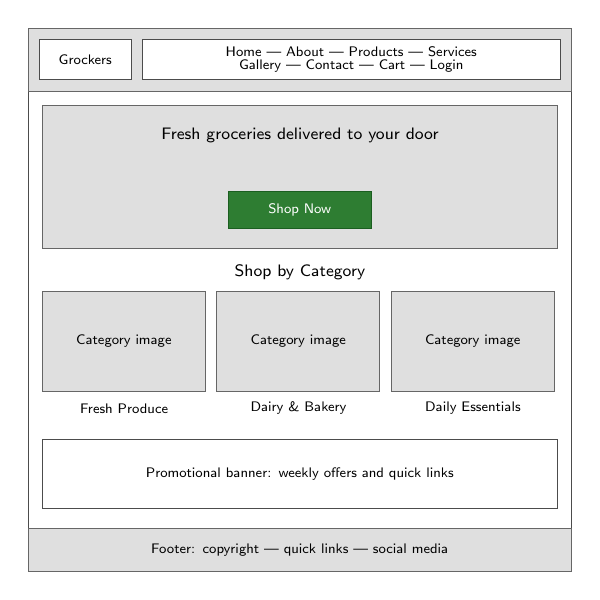
\begin{tikzpicture}
\wb{0.000}{0.000}{6.900}{6.900}{wfbox}{4.13}{4.96}{6.860}{}
\wb{0.000}{6.101}{6.900}{0.799}{wffill}{4.13}{4.96}{6.860}{}
\wb{0.145}{6.246}{1.162}{0.508}{wfbox}{4.65}{5.58}{1.122}{Grockers}
\wb{1.453}{6.246}{5.302}{0.508}{wfbox}{4.13}{4.96}{5.262}{Home | About | Products | Services \\ Gallery | Contact | Cart | Login}
\wb{0.000}{0.000}{6.900}{0.545}{wffill}{4.13}{4.96}{6.860}{Footer: copyright | quick links | social media}
\wb{0.182}{4.104}{6.537}{1.816}{wffill}{5.17}{6.20}{6.497}{}
\wb{0.182}{5.302}{6.537}{0.472}{wfbold}{5.68}{6.82}{6.497}{Fresh groceries delivered to your door}
\wb{2.542}{4.358}{1.816}{0.472}{wfbtn}{5.17}{6.20}{1.776}{Shop Now}
\wb{0.182}{3.632}{6.537}{0.327}{wfbold}{5.68}{6.82}{6.497}{Shop by Category}
\wb{0.182}{2.288}{2.070}{1.271}{wffill}{4.65}{5.58}{2.030}{Category image}
\wb{0.182}{1.925}{2.070}{0.291}{wftext}{5.17}{6.20}{2.030}{Fresh Produce}
\wb{2.397}{2.288}{2.070}{1.271}{wffill}{4.65}{5.58}{2.030}{Category image}
\wb{2.397}{1.925}{2.070}{0.291}{wftext}{5.17}{6.20}{2.030}{Dairy \& Bakery}
\wb{4.612}{2.288}{2.070}{1.271}{wffill}{4.65}{5.58}{2.030}{Category image}
\wb{4.612}{1.925}{2.070}{0.291}{wftext}{5.17}{6.20}{2.030}{Daily Essentials}
\wb{0.182}{0.799}{6.537}{0.872}{wfbox}{5.17}{6.20}{6.497}{Promotional banner: weekly offers and quick links}
\end{tikzpicture}
\captionof{figure}{Wireframe of the Home page (\texttt{index.html})}\label{fig:wf-home}\end{minipage}\hfill
\begin{minipage}[t]{0.485\textwidth}\centering
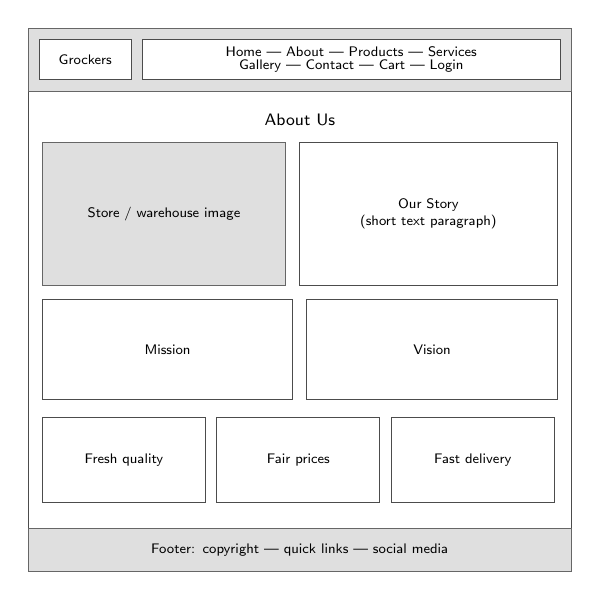
\begin{tikzpicture}
\wb{0.000}{0.000}{6.900}{6.900}{wfbox}{4.13}{4.96}{6.860}{}
\wb{0.000}{6.101}{6.900}{0.799}{wffill}{4.13}{4.96}{6.860}{}
\wb{0.145}{6.246}{1.162}{0.508}{wfbox}{4.65}{5.58}{1.122}{Grockers}
\wb{1.453}{6.246}{5.302}{0.508}{wfbox}{4.13}{4.96}{5.262}{Home | About | Products | Services \\ Gallery | Contact | Cart | Login}
\wb{0.000}{0.000}{6.900}{0.545}{wffill}{4.13}{4.96}{6.860}{Footer: copyright | quick links | social media}
\wb{0.182}{5.556}{6.537}{0.363}{wfbold}{6.20}{7.44}{6.497}{About Us}
\wb{0.182}{3.632}{3.087}{1.816}{wffill}{5.17}{6.20}{3.047}{Store / warehouse image}
\wb{3.450}{3.632}{3.268}{1.816}{wfbox}{5.17}{6.20}{3.228}{Our Story \\ (short text paragraph)}
\wb{0.182}{2.179}{3.178}{1.271}{wfbox}{5.17}{6.20}{3.138}{Mission}
\wb{3.541}{2.179}{3.178}{1.271}{wfbox}{5.17}{6.20}{3.138}{Vision}
\wb{0.182}{0.872}{2.070}{1.089}{wfbox}{5.17}{6.20}{2.030}{Fresh quality}
\wb{2.397}{0.872}{2.070}{1.089}{wfbox}{5.17}{6.20}{2.030}{Fair prices}
\wb{4.612}{0.872}{2.070}{1.089}{wfbox}{5.17}{6.20}{2.030}{Fast delivery}
\end{tikzpicture}
\captionof{figure}{Wireframe of the About Us page (\texttt{about.html})}\label{fig:wf-about}\end{minipage}

\medskip
\begin{minipage}[t]{0.485\textwidth}\centering
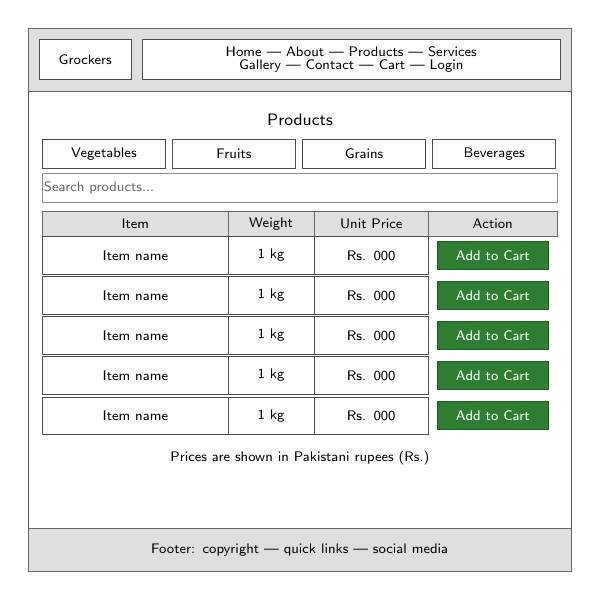
\begin{tikzpicture}
\wb{0.000}{0.000}{6.900}{6.900}{wfbox}{4.13}{4.96}{6.860}{}
\wb{0.000}{6.101}{6.900}{0.799}{wffill}{4.13}{4.96}{6.860}{}
\wb{0.145}{6.246}{1.162}{0.508}{wfbox}{4.65}{5.58}{1.122}{Grockers}
\wb{1.453}{6.246}{5.302}{0.508}{wfbox}{4.13}{4.96}{5.262}{Home | About | Products | Services \\ Gallery | Contact | Cart | Login}
\wb{0.000}{0.000}{6.900}{0.545}{wffill}{4.13}{4.96}{6.860}{Footer: copyright | quick links | social media}
\wb{0.182}{5.556}{6.537}{0.363}{wfbold}{6.20}{7.44}{6.497}{Products}
\wb{0.182}{5.121}{1.562}{0.363}{wfbox}{4.65}{5.58}{1.522}{Vegetables}
\wb{1.834}{5.121}{1.562}{0.363}{wfbox}{4.65}{5.58}{1.522}{Fruits}
\wb{3.486}{5.121}{1.562}{0.363}{wfbox}{4.65}{5.58}{1.522}{Grains}
\wb{5.139}{5.121}{1.562}{0.363}{wfbox}{4.65}{5.58}{1.522}{Beverages}
\wb{0.182}{4.685}{6.537}{0.363}{wfinput}{4.65}{5.58}{6.497}{Search products...}
\wb{0.182}{4.249}{2.361}{0.327}{wffill}{4.65}{5.58}{2.321}{Item}
\wb{2.542}{4.249}{1.089}{0.327}{wffill}{4.65}{5.58}{1.049}{Weight}
\wb{3.632}{4.249}{1.453}{0.327}{wffill}{4.65}{5.58}{1.413}{Unit Price}
\wb{5.084}{4.249}{1.634}{0.327}{wffill}{4.65}{5.58}{1.594}{Action}
\wb{0.182}{3.777}{2.361}{0.472}{wfbox}{4.65}{5.58}{2.321}{Item name}
\wb{2.542}{3.777}{1.089}{0.472}{wfbox}{4.65}{5.58}{1.049}{1 kg}
\wb{3.632}{3.777}{1.453}{0.472}{wfbox}{4.65}{5.58}{1.413}{Rs. 000}
\wb{5.193}{3.831}{1.416}{0.363}{wfbtn}{4.13}{4.96}{1.376}{Add to Cart}
\wb{0.182}{3.268}{2.361}{0.472}{wfbox}{4.65}{5.58}{2.321}{Item name}
\wb{2.542}{3.268}{1.089}{0.472}{wfbox}{4.65}{5.58}{1.049}{1 kg}
\wb{3.632}{3.268}{1.453}{0.472}{wfbox}{4.65}{5.58}{1.413}{Rs. 000}
\wb{5.193}{3.323}{1.416}{0.363}{wfbtn}{4.13}{4.96}{1.376}{Add to Cart}
\wb{0.182}{2.760}{2.361}{0.472}{wfbox}{4.65}{5.58}{2.321}{Item name}
\wb{2.542}{2.760}{1.089}{0.472}{wfbox}{4.65}{5.58}{1.049}{1 kg}
\wb{3.632}{2.760}{1.453}{0.472}{wfbox}{4.65}{5.58}{1.413}{Rs. 000}
\wb{5.193}{2.814}{1.416}{0.363}{wfbtn}{4.13}{4.96}{1.376}{Add to Cart}
\wb{0.182}{2.252}{2.361}{0.472}{wfbox}{4.65}{5.58}{2.321}{Item name}
\wb{2.542}{2.252}{1.089}{0.472}{wfbox}{4.65}{5.58}{1.049}{1 kg}
\wb{3.632}{2.252}{1.453}{0.472}{wfbox}{4.65}{5.58}{1.413}{Rs. 000}
\wb{5.193}{2.306}{1.416}{0.363}{wfbtn}{4.13}{4.96}{1.376}{Add to Cart}
\wb{0.182}{1.743}{2.361}{0.472}{wfbox}{4.65}{5.58}{2.321}{Item name}
\wb{2.542}{1.743}{1.089}{0.472}{wfbox}{4.65}{5.58}{1.049}{1 kg}
\wb{3.632}{1.743}{1.453}{0.472}{wfbox}{4.65}{5.58}{1.413}{Rs. 000}
\wb{5.193}{1.798}{1.416}{0.363}{wfbtn}{4.13}{4.96}{1.376}{Add to Cart}
\wb{0.182}{1.271}{6.537}{0.327}{wftext}{4.13}{4.96}{6.497}{Prices are shown in Pakistani rupees (Rs.)}
\end{tikzpicture}
\captionof{figure}{Wireframe of the Products page (\texttt{products.html})}\label{fig:wf-products}\end{minipage}\hfill
\begin{minipage}[t]{0.485\textwidth}\centering
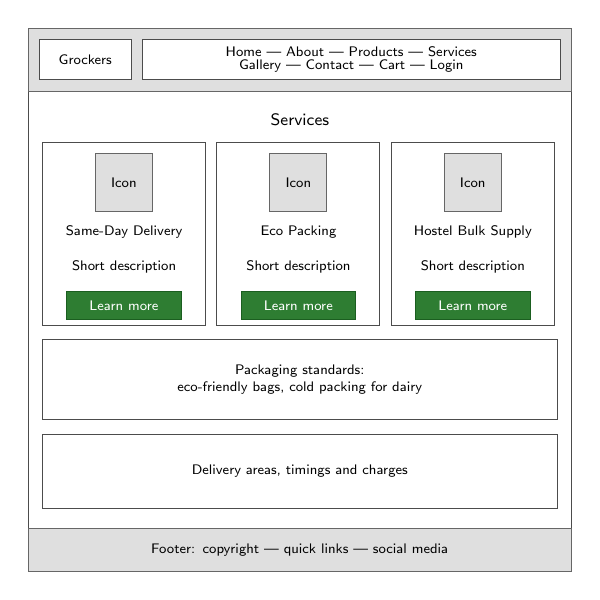
\begin{tikzpicture}
\wb{0.000}{0.000}{6.900}{6.900}{wfbox}{4.13}{4.96}{6.860}{}
\wb{0.000}{6.101}{6.900}{0.799}{wffill}{4.13}{4.96}{6.860}{}
\wb{0.145}{6.246}{1.162}{0.508}{wfbox}{4.65}{5.58}{1.122}{Grockers}
\wb{1.453}{6.246}{5.302}{0.508}{wfbox}{4.13}{4.96}{5.262}{Home | About | Products | Services \\ Gallery | Contact | Cart | Login}
\wb{0.000}{0.000}{6.900}{0.545}{wffill}{4.13}{4.96}{6.860}{Footer: copyright | quick links | social media}
\wb{0.182}{5.556}{6.537}{0.363}{wfbold}{6.20}{7.44}{6.497}{Services}
\wb{0.182}{3.123}{2.070}{2.324}{wfbox}{4.65}{5.58}{2.030}{}
\wb{0.853}{4.576}{0.726}{0.726}{wffill}{4.65}{5.58}{0.686}{Icon}
\wb{0.182}{4.140}{2.070}{0.327}{wfbold}{4.65}{5.58}{2.030}{Same-Day Delivery}
\wb{0.182}{3.632}{2.070}{0.472}{wftext}{4.65}{5.58}{2.030}{Short description}
\wb{0.490}{3.196}{1.453}{0.363}{wfbtn}{4.13}{4.96}{1.413}{Learn more}
\wb{2.397}{3.123}{2.070}{2.324}{wfbox}{4.65}{5.58}{2.030}{}
\wb{3.069}{4.576}{0.726}{0.726}{wffill}{4.65}{5.58}{0.686}{Icon}
\wb{2.397}{4.140}{2.070}{0.327}{wfbold}{4.65}{5.58}{2.030}{Eco Packing}
\wb{2.397}{3.632}{2.070}{0.472}{wftext}{4.65}{5.58}{2.030}{Short description}
\wb{2.706}{3.196}{1.453}{0.363}{wfbtn}{4.13}{4.96}{1.413}{Learn more}
\wb{4.612}{3.123}{2.070}{2.324}{wfbox}{4.65}{5.58}{2.030}{}
\wb{5.284}{4.576}{0.726}{0.726}{wffill}{4.65}{5.58}{0.686}{Icon}
\wb{4.612}{4.140}{2.070}{0.327}{wfbold}{4.65}{5.58}{2.030}{Hostel Bulk Supply}
\wb{4.612}{3.632}{2.070}{0.472}{wftext}{4.65}{5.58}{2.030}{Short description}
\wb{4.921}{3.196}{1.453}{0.363}{wfbtn}{4.13}{4.96}{1.413}{Learn more}
\wb{0.182}{1.925}{6.537}{1.017}{wfbox}{5.17}{6.20}{6.497}{Packaging standards: \\ eco-friendly bags, cold packing for dairy}
\wb{0.182}{0.799}{6.537}{0.944}{wfbox}{5.17}{6.20}{6.497}{Delivery areas, timings and charges}
\end{tikzpicture}
\captionof{figure}{Wireframe of the Services page (\texttt{services.html})}\label{fig:wf-services}\end{minipage}

\medskip
\begin{minipage}[t]{0.485\textwidth}\centering
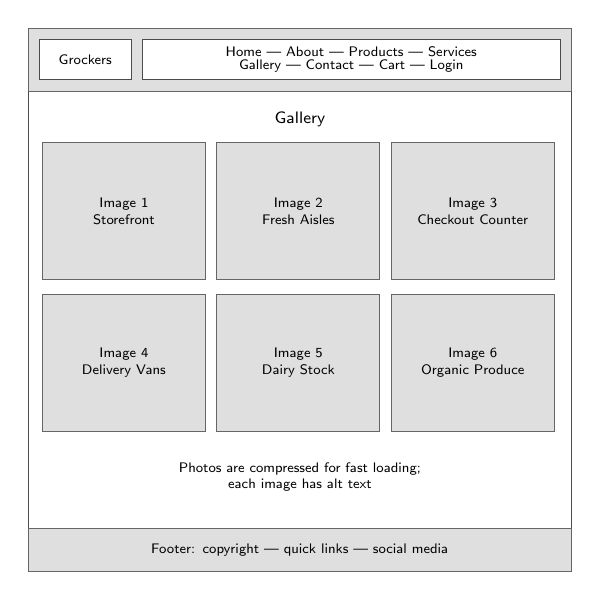
\begin{tikzpicture}
\wb{0.000}{0.000}{6.900}{6.900}{wfbox}{4.13}{4.96}{6.860}{}
\wb{0.000}{6.101}{6.900}{0.799}{wffill}{4.13}{4.96}{6.860}{}
\wb{0.145}{6.246}{1.162}{0.508}{wfbox}{4.65}{5.58}{1.122}{Grockers}
\wb{1.453}{6.246}{5.302}{0.508}{wfbox}{4.13}{4.96}{5.262}{Home | About | Products | Services \\ Gallery | Contact | Cart | Login}
\wb{0.000}{0.000}{6.900}{0.545}{wffill}{4.13}{4.96}{6.860}{Footer: copyright | quick links | social media}
\wb{0.182}{5.556}{6.537}{0.363}{wfbold}{6.20}{7.44}{6.497}{Gallery}
\wb{0.182}{3.704}{2.070}{1.743}{wffill}{5.17}{6.20}{2.030}{Image 1 \\ Storefront}
\wb{2.397}{3.704}{2.070}{1.743}{wffill}{5.17}{6.20}{2.030}{Image 2 \\ Fresh Aisles}
\wb{4.612}{3.704}{2.070}{1.743}{wffill}{5.17}{6.20}{2.030}{Image 3 \\ Checkout Counter}
\wb{0.182}{1.779}{2.070}{1.743}{wffill}{5.17}{6.20}{2.030}{Image 4 \\ Delivery Vans}
\wb{2.397}{1.779}{2.070}{1.743}{wffill}{5.17}{6.20}{2.030}{Image 5 \\ Dairy Stock}
\wb{4.612}{1.779}{2.070}{1.743}{wffill}{5.17}{6.20}{2.030}{Image 6 \\ Organic Produce}
\wb{0.182}{0.872}{6.537}{0.654}{wftext}{4.65}{5.58}{6.497}{Photos are compressed for fast loading; \\ each image has alt text}
\end{tikzpicture}
\captionof{figure}{Wireframe of the Gallery page (\texttt{gallery.html})}\label{fig:wf-gallery}\end{minipage}\hfill
\begin{minipage}[t]{0.485\textwidth}\centering
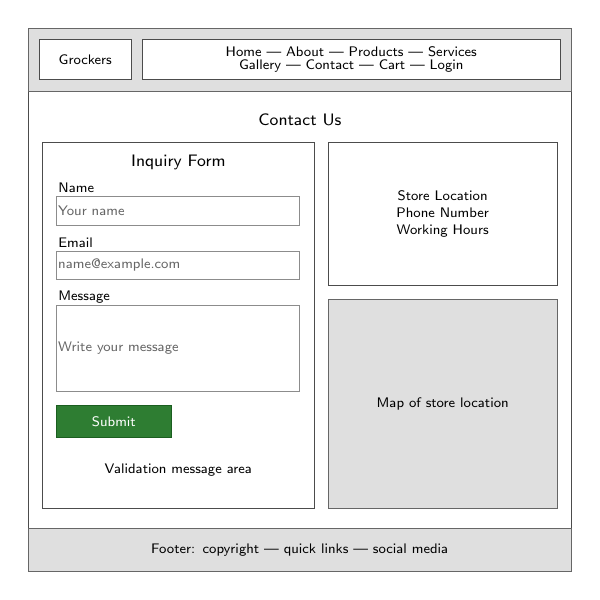
\begin{tikzpicture}
\wb{0.000}{0.000}{6.900}{6.900}{wfbox}{4.13}{4.96}{6.860}{}
\wb{0.000}{6.101}{6.900}{0.799}{wffill}{4.13}{4.96}{6.860}{}
\wb{0.145}{6.246}{1.162}{0.508}{wfbox}{4.65}{5.58}{1.122}{Grockers}
\wb{1.453}{6.246}{5.302}{0.508}{wfbox}{4.13}{4.96}{5.262}{Home | About | Products | Services \\ Gallery | Contact | Cart | Login}
\wb{0.000}{0.000}{6.900}{0.545}{wffill}{4.13}{4.96}{6.860}{Footer: copyright | quick links | social media}
\wb{0.182}{5.556}{6.537}{0.363}{wfbold}{6.20}{7.44}{6.497}{Contact Us}
\wb{0.182}{0.799}{3.450}{4.648}{wfbox}{4.65}{5.58}{3.410}{}
\wb{0.363}{5.048}{3.087}{0.291}{wfbold}{5.68}{6.82}{3.047}{Inquiry Form}
\wb{0.363}{4.757}{3.087}{0.218}{wflbl}{4.65}{5.58}{3.047}{Name}
\wb{0.363}{4.394}{3.087}{0.363}{wfinput}{4.65}{5.58}{3.047}{Your name}
\wb{0.363}{4.067}{3.087}{0.218}{wflbl}{4.65}{5.58}{3.047}{Email}
\wb{0.363}{3.704}{3.087}{0.363}{wfinput}{4.65}{5.58}{3.047}{name@example.com}
\wb{0.363}{3.377}{3.087}{0.218}{wflbl}{4.65}{5.58}{3.047}{Message}
\wb{0.363}{2.288}{3.087}{1.089}{wfinput}{4.65}{5.58}{3.047}{Write your message}
\wb{0.363}{1.707}{1.453}{0.399}{wfbtn}{4.65}{5.58}{1.413}{Submit}
\wb{0.363}{1.017}{3.087}{0.545}{wftext}{4.13}{4.96}{3.047}{Validation message area}
\wb{3.813}{3.632}{2.905}{1.816}{wfbox}{5.17}{6.20}{2.865}{Store Location \\ Phone Number \\ Working Hours}
\wb{3.813}{0.799}{2.905}{2.651}{wffill}{5.17}{6.20}{2.865}{Map of store location}
\end{tikzpicture}
\captionof{figure}{Wireframe of the Contact Us page (\texttt{contact.html})}\label{fig:wf-contact}\end{minipage}

\clearpage
\begin{minipage}[t]{0.485\textwidth}\centering
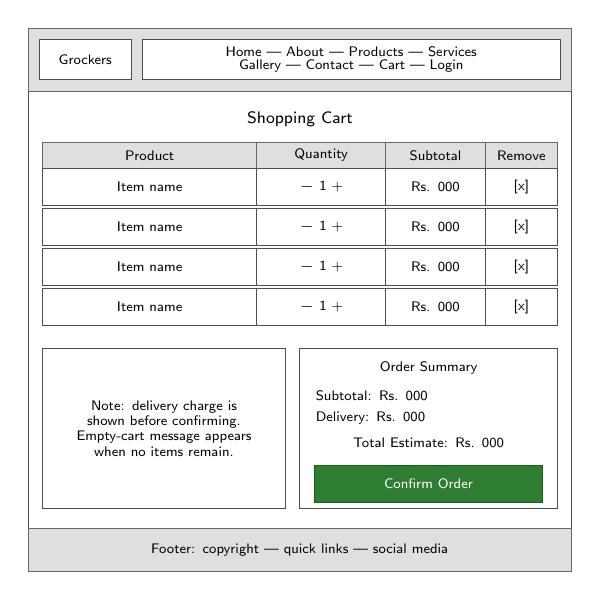
\begin{tikzpicture}
\wb{0.000}{0.000}{6.900}{6.900}{wfbox}{4.13}{4.96}{6.860}{}
\wb{0.000}{6.101}{6.900}{0.799}{wffill}{4.13}{4.96}{6.860}{}
\wb{0.145}{6.246}{1.162}{0.508}{wfbox}{4.65}{5.58}{1.122}{Grockers}
\wb{1.453}{6.246}{5.302}{0.508}{wfbox}{4.13}{4.96}{5.262}{Home | About | Products | Services \\ Gallery | Contact | Cart | Login}
\wb{0.000}{0.000}{6.900}{0.545}{wffill}{4.13}{4.96}{6.860}{Footer: copyright | quick links | social media}
\wb{0.182}{5.556}{6.537}{0.363}{wfbold}{6.20}{7.44}{6.497}{Shopping Cart}
\wb{0.182}{5.121}{2.724}{0.327}{wffill}{4.65}{5.58}{2.684}{Product}
\wb{2.905}{5.121}{1.634}{0.327}{wffill}{4.65}{5.58}{1.594}{Quantity}
\wb{4.539}{5.121}{1.271}{0.327}{wffill}{4.65}{5.58}{1.231}{Subtotal}
\wb{5.811}{5.121}{0.908}{0.327}{wffill}{4.65}{5.58}{0.868}{Remove}
\wb{0.182}{4.648}{2.724}{0.472}{wfbox}{4.65}{5.58}{2.684}{Item name}
\wb{2.905}{4.648}{1.634}{0.472}{wfbox}{4.65}{5.58}{1.594}{$-$  1  +}
\wb{4.539}{4.648}{1.271}{0.472}{wfbox}{4.65}{5.58}{1.231}{Rs. 000}
\wb{5.811}{4.648}{0.908}{0.472}{wfbox}{4.65}{5.58}{0.868}{[x]}
\wb{0.182}{4.140}{2.724}{0.472}{wfbox}{4.65}{5.58}{2.684}{Item name}
\wb{2.905}{4.140}{1.634}{0.472}{wfbox}{4.65}{5.58}{1.594}{$-$  1  +}
\wb{4.539}{4.140}{1.271}{0.472}{wfbox}{4.65}{5.58}{1.231}{Rs. 000}
\wb{5.811}{4.140}{0.908}{0.472}{wfbox}{4.65}{5.58}{0.868}{[x]}
\wb{0.182}{3.632}{2.724}{0.472}{wfbox}{4.65}{5.58}{2.684}{Item name}
\wb{2.905}{3.632}{1.634}{0.472}{wfbox}{4.65}{5.58}{1.594}{$-$  1  +}
\wb{4.539}{3.632}{1.271}{0.472}{wfbox}{4.65}{5.58}{1.231}{Rs. 000}
\wb{5.811}{3.632}{0.908}{0.472}{wfbox}{4.65}{5.58}{0.868}{[x]}
\wb{0.182}{3.123}{2.724}{0.472}{wfbox}{4.65}{5.58}{2.684}{Item name}
\wb{2.905}{3.123}{1.634}{0.472}{wfbox}{4.65}{5.58}{1.594}{$-$  1  +}
\wb{4.539}{3.123}{1.271}{0.472}{wfbox}{4.65}{5.58}{1.231}{Rs. 000}
\wb{5.811}{3.123}{0.908}{0.472}{wfbox}{4.65}{5.58}{0.868}{[x]}
\wb{0.182}{0.799}{3.087}{2.034}{wfbox}{4.65}{5.58}{3.047}{Note: delivery charge is \\ shown before confirming. \\ Empty-cart message appears \\ when no items remain.}
\wb{3.450}{0.799}{3.268}{2.034}{wfbox}{4.65}{5.58}{3.228}{}
\wb{3.632}{2.433}{2.905}{0.291}{wfbold}{5.17}{6.20}{2.865}{Order Summary}
\wb{3.632}{2.106}{2.905}{0.254}{wflbl}{4.65}{5.58}{2.865}{Subtotal: Rs. 000}
\wb{3.632}{1.816}{2.905}{0.254}{wflbl}{4.65}{5.58}{2.865}{Delivery: Rs. 000}
\wb{3.632}{1.489}{2.905}{0.291}{wfbold}{4.65}{5.58}{2.865}{Total Estimate: Rs. 000}
\wb{3.632}{0.872}{2.905}{0.472}{wfbtn}{4.65}{5.58}{2.865}{Confirm Order}
\end{tikzpicture}
\captionof{figure}{Wireframe of the Shopping Cart page (\texttt{cart.html})}\label{fig:wf-cart}\end{minipage}\hfill
\begin{minipage}[t]{0.485\textwidth}\centering
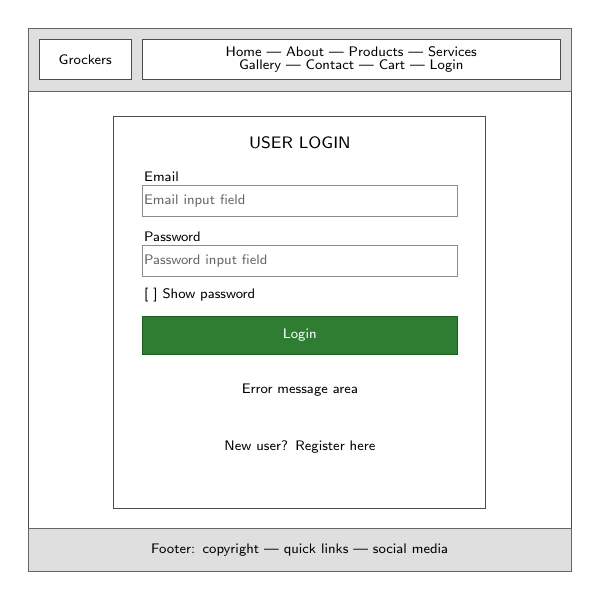
\begin{tikzpicture}
\wb{0.000}{0.000}{6.900}{6.900}{wfbox}{4.13}{4.96}{6.860}{}
\wb{0.000}{6.101}{6.900}{0.799}{wffill}{4.13}{4.96}{6.860}{}
\wb{0.145}{6.246}{1.162}{0.508}{wfbox}{4.65}{5.58}{1.122}{Grockers}
\wb{1.453}{6.246}{5.302}{0.508}{wfbox}{4.13}{4.96}{5.262}{Home | About | Products | Services \\ Gallery | Contact | Cart | Login}
\wb{0.000}{0.000}{6.900}{0.545}{wffill}{4.13}{4.96}{6.860}{Footer: copyright | quick links | social media}
\wb{1.089}{0.799}{4.721}{4.975}{wfbox}{4.65}{5.58}{4.681}{}
\wb{1.089}{5.266}{4.721}{0.363}{wfbold}{6.20}{7.44}{4.681}{USER LOGIN}
\wb{1.453}{4.903}{3.995}{0.218}{wflbl}{4.65}{5.58}{3.955}{Email}
\wb{1.453}{4.503}{3.995}{0.399}{wfinput}{4.65}{5.58}{3.955}{Email input field}
\wb{1.453}{4.140}{3.995}{0.218}{wflbl}{4.65}{5.58}{3.955}{Password}
\wb{1.453}{3.741}{3.995}{0.399}{wfinput}{4.65}{5.58}{3.955}{Password input field}
\wb{1.453}{3.377}{3.995}{0.254}{wflbl}{4.13}{4.96}{3.955}{[ ] Show password}
\wb{1.453}{2.760}{3.995}{0.472}{wfbtn}{5.17}{6.20}{3.955}{Login}
\wb{1.453}{2.034}{3.995}{0.545}{wftext}{4.13}{4.96}{3.955}{Error message area}
\wb{1.453}{1.416}{3.995}{0.327}{wftext}{4.65}{5.58}{3.955}{New user? Register here}
\end{tikzpicture}
\captionof{figure}{Wireframe of the Login page (\texttt{login.html})}\label{fig:wf-login}\end{minipage}

\medskip
\begin{minipage}[t]{0.485\textwidth}\centering
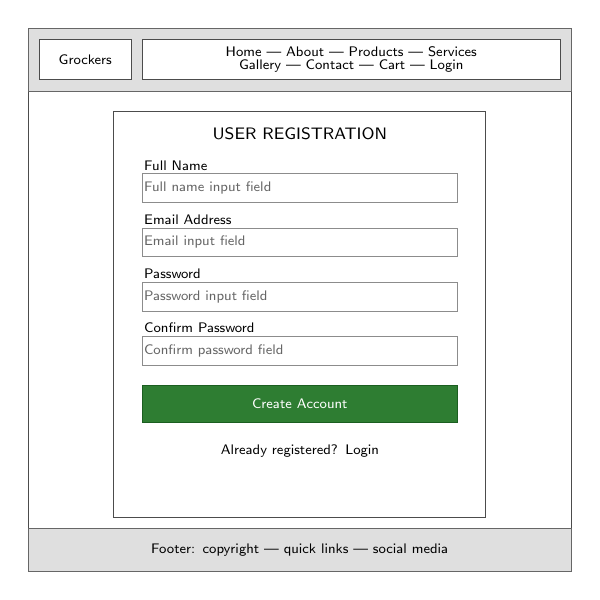
\begin{tikzpicture}
\wb{0.000}{0.000}{6.900}{6.900}{wfbox}{4.13}{4.96}{6.860}{}
\wb{0.000}{6.101}{6.900}{0.799}{wffill}{4.13}{4.96}{6.860}{}
\wb{0.145}{6.246}{1.162}{0.508}{wfbox}{4.65}{5.58}{1.122}{Grockers}
\wb{1.453}{6.246}{5.302}{0.508}{wfbox}{4.13}{4.96}{5.262}{Home | About | Products | Services \\ Gallery | Contact | Cart | Login}
\wb{0.000}{0.000}{6.900}{0.545}{wffill}{4.13}{4.96}{6.860}{Footer: copyright | quick links | social media}
\wb{1.089}{0.690}{4.721}{5.157}{wfbox}{4.65}{5.58}{4.681}{}
\wb{1.089}{5.375}{4.721}{0.363}{wfbold}{6.20}{7.44}{4.681}{USER REGISTRATION}
\wb{1.453}{5.048}{3.995}{0.218}{wflbl}{4.65}{5.58}{3.955}{Full Name}
\wb{1.453}{4.685}{3.995}{0.363}{wfinput}{4.65}{5.58}{3.955}{Full name input field}
\wb{1.453}{4.358}{3.995}{0.218}{wflbl}{4.65}{5.58}{3.955}{Email Address}
\wb{1.453}{3.995}{3.995}{0.363}{wfinput}{4.65}{5.58}{3.955}{Email input field}
\wb{1.453}{3.668}{3.995}{0.218}{wflbl}{4.65}{5.58}{3.955}{Password}
\wb{1.453}{3.305}{3.995}{0.363}{wfinput}{4.65}{5.58}{3.955}{Password input field}
\wb{1.453}{2.978}{3.995}{0.218}{wflbl}{4.65}{5.58}{3.955}{Confirm Password}
\wb{1.453}{2.615}{3.995}{0.363}{wfinput}{4.65}{5.58}{3.955}{Confirm password field}
\wb{1.453}{1.888}{3.995}{0.472}{wfbtn}{5.17}{6.20}{3.955}{Create Account}
\wb{1.453}{1.380}{3.995}{0.291}{wftext}{4.65}{5.58}{3.955}{Already registered? Login}
\end{tikzpicture}
\captionof{figure}{Wireframe of the Sign-Up page (\texttt{signup.html})}\label{fig:wf-signup}\end{minipage}\hfill
\begin{minipage}[t]{0.485\textwidth}
\vspace{0pt}
\captionof{table}{Responsive breakpoints used for the layouts}\label{tab:bp}
\tbl
\begin{tabularx}{\linewidth}{@{}lYl@{}}
\rowcolor{gkgreen}\hc{Screen} & \hc{Layout} & \hc{Width}\\
Phone & One column; menu collapses into a button; tables scroll inside their box. & 360--599 px\\
Tablet & Two columns for cards and the gallery; full navigation bar. & 600--991 px\\
Desktop & Three to four columns; wireframes above show this layout. & 992 px and up\\
\end{tabularx}
\end{minipage}

\subsection{Folder Structure}
All files are kept in one GitHub repository. Names use lowercase letters and hyphens only, so links work on every operating system.
\begin{center}
\fbox{\begin{minipage}{0.72\textwidth}
\ttfamily\footnotesize
grockers-website/\\
\textbar-- index.html, about.html, products.html\\
\textbar-- services.html, gallery.html, contact.html\\
\textbar-- cart.html, login.html, signup.html\\
\textbar-- css/\ \ \ (style.css)\\
\textbar-- js/\ \ \ \ \ (main.js, validation.js)\\
\textbar-- images/\\
\textbar-- wireframes/\ \ (wireframes.drawio, PNG exports)\\
\textbackslash-- README.md
\end{minipage}}
\end{center}

\subsection{Tools}
\begin{table}[H]
\centering
\caption{Tools used in the project}
\tbl
\begin{tabularx}{\textwidth}{@{}lY@{}}
\rowcolor{gkgreen}\hc{Tool} & \hc{Use}\\
Visual Studio Code & Writing HTML, CSS and JavaScript\\
Chrome / Firefox / Edge & Testing and developer tools\\
Git and GitHub & Version control, teamwork and GitHub Pages hosting\\
Overleaf (LaTeX) & Writing the project report together\\
draw.io & Site map and wireframes\\
W3C validators & Checking HTML and CSS\\
\end{tabularx}
\end{table}

\subsection{Team Task Allocation}
\begin{table}[H]
\centering
\caption{Team roles and task distribution}
\tbl
\begin{tabularx}{\textwidth}{@{}llY@{}}
\rowcolor{gkgreen}\hc{Team member} & \hc{Role} & \hc{Responsibilities}\\
Ghulam Qadir & HTML developer and basic CSS & Builds the base structure of all HTML pages with semantic tags; writes the first half of the CSS: colours, fonts and layout styling.\\
Asaam Abdullah & Report writer and designer & Adds content, lists and tables to the HTML pages; writes the LaTeX report (Chapters 1--3) on Overleaf; manages the site map and wireframes.\\
Armish Malik & Responsive CSS, JavaScript and GitHub & Writes the second half of the CSS (Flexbox/Grid, media queries); JavaScript form validation and interactive features; manages the GitHub repository (commits and README).\\
\end{tabularx}
\end{table}

\subsection{Time Plan}
\begin{table}[H]
\centering
\caption{Time plan up to the final deadline}
\tbl
\begin{tabularx}{\textwidth}{@{}lcYl@{}}
\rowcolor{gkgreen}\hc{Dates} & \hc{Phase} & \hc{Work (by member)} & \hc{Milestone}\\
16--19 Nov & 1 & Asaam: Chapters 1--3, site map, wireframes. Armish: GitHub repository, README, wireframe images. Ghulam: plans HTML page structure. & Deliverable 1 due 19/11\\
20--26 Nov & 2 & Ghulam: semantic HTML for all pages, basic CSS. Asaam: adds content, lists and tables; Chapter 4. Armish: responsive CSS, W3C validation, commits. & Deliverable 2 due 26/11\\
27 Nov--3 Dec & 3 & Armish: JavaScript form validation, cart and other interactive features. Ghulam: fixes HTML/CSS issues found. Asaam: Chapters 5--6 drafts. & Features complete\\
4--10 Dec & 3 & All: testing (10+ test cases), bug fixes, GitHub Pages, LinkedIn video. Asaam completes the report. & Final deliverable due 10/12\\
11--17 Dec & 3 & All: practise the demo. & Demo and viva 17/12\\
\end{tabularx}
\end{table}

\subsection{Risks and Mitigation}
\begin{table}[H]
\centering
\caption{Main project risks}
\tbl
\begin{tabularx}{\textwidth}{@{}YlY@{}}
\rowcolor{gkgreen}\hc{Risk} & \hc{Level} & \hc{Mitigation}\\
Merge conflicts in shared CSS or HTML files & Medium & Pull before every push; small, frequent commits; each member edits their own CSS section.\\
Slow pages caused by large images & Medium & Compress images (JPEG/WebP, under about 200 KB each) and check load time in developer tools.\\
Validation errors found too late & Medium & Run the W3C validators after finishing each page, not only at the end.\\
Uneven workload or a member unavailable & Low & Short weekly check-in; every task has a named backup member.\\
\end{tabularx}
\end{table}

\end{document}
